\documentclass[sigconf]{acmart}

%\usepackage{booktabs} % For formal tables
\usepackage{listings}
\usepackage{todonotes}
\usepackage{hyperref}
\usepackage{algorithm}
\usepackage{algorithmic}
\usepackage{balance}
\usepackage{footmisc}

\begin{document}
\title{Scaling Column Imprints using Advanced Vectorization}

\author{Lefteris Sidirourgos}
\authornote{this work was done while the author was at CWI.}
\affiliation{%
  \institution{Systems Group\\Dept. of Computer Science\\ETH Zurich, Switzerland}
}
\email{lsidir@inf.ethz.ch}

\author{Hannes M\"uhleisen}
\affiliation{%
  \institution{Database Architectures Group\\Centrum Wiskunde \& Informatica}
  \streetaddress{Amsterdam, The Netherlands}
}
\email{hannes@cwi.nl}

\copyrightyear{2017}
\acmYear{2017} 
\setcopyright{acmcopyright}
\acmConference{DaMoN'17}{May       15, 2017}{Chicago, IL, USA}\acmPrice{15.00}\acmDOI{http://dx.doi.org/10.1145/3076113.3076120}
\acmISBN{978-1-4503-5025-9/17/05}

\lstset{basicstyle=\ttfamily}


\begin{abstract}
{\em Column Imprints} is a pre-filtering secondary index for answering range queries. The main feature of imprints is that they are
lightweight and are based on compressed bit-vectors, one per cacheline, that quickly determine if the values in that cacheline 
satisfy the predicates of a query. The main overhead of the imprints implementation is the many sequential value comparisons against 
the boundaries of a virtual equi-height histogram. Similarly, during query scans, many sequential value comparisons are performed to
identify false positives. In this paper, we speed-up the process of imprints creation and querying by using advanced vectorization 
techniques. We also experimentally explore the benefits of stretching imprints to larger bit-vector sizes and blocks of data, using
256-bit SIMD registers. Our findings are very promising for both imprints and for future index design research that would employ 
advanced vectorization techniques and larger (up to 512-bit) and more (from 16 now to 32) SIMD registers.

\end{abstract}

\begin{CCSXML}
<ccs2012>
<concept>
<concept_id>10002951.10002952.10003190.10003192</concept_id>
<concept_desc>Information systems~Database query processing</concept_desc>
<concept_significance>500</concept_significance>
</concept>
<concept>
<concept_id>10002951.10002952.10002971.10003450.10010828</concept_id>
<concept_desc>Information systems~Data scans</concept_desc>
<concept_significance>500</concept_significance>
</concept>
</ccs2012>
\end{CCSXML}

\ccsdesc[500]{Information systems ~ Database query processing}
\ccsdesc[500]{Information systems ~ Data scans}


%\keywords{ACM proceedings, \LaTeX, text tagging}


\maketitle

\section{Introduction}

{\em Column Imprints}~\cite{DBLP:conf/sigmod/SidirourgosK13} is a secondary index
for answering range queries in a read optimized columnar database. Imprints are
pre-filtering bit-vectors that quickly determine if a cache line or block of data
contains values that satisfy the range predicates of a query. They have been designed
such that they are easy to build, typically as a side effect of the first range-scan query,
and then subsequently used by all other queries. The imprints index structure is simple
and lightweight, never exceeding 12\% of the original size of the column, while speeding
up significantly query execution times. {\em Column Imprints} are particularly useful for those
attributes that are on the tail of a relational table, not worth the investment of building
a primary (sort/cluster) index, yet often part of the many range predicates of a query.

{\em Column Imprints} are so efficient because they are built during a single 
sequential scan, where each value is compared against a number of boundaries
of an equi-height histogram, in order to set the corresponding bit on a small bit-vector.
An imprint is typically only 64-bits and stored as an unsigned long. Similarly,
during query time, one sequential scan is needed over the imprints to quickly determine
which blocks of data qualify for query evaluation. Even with such short description of
the creation and usage of imprints, it is easy to assume that a vectorized programming
framework with native CPU support will greatly benefit the performance of the index.

In this paper we make use of Intel's Advanced Vector Extensions 
\cite{IntelManual2011} to speed up {\em Column Imprints}. SIMD instructions are used 
{\em i)} to efficiently compare multiple values against histogram boundaries, {\em ii)} to perform 
multiple bit-wise operations over imprints that extend beyond the
standard 64-bit unsigned long words, and {\em iii)} to filter out false positive 
values at query time. These three points are the main computation intensive parts
of the  creation and query process of the index, and are exactly the ones that should be 
optimized by vectorization. As we will describe in detail in the next section, 
{\em Column Imprints} also employ compression techniques and dictionary-style bookkeeping,
but these parts of the code are less often invoked and have many control-flow branching 
making them unsuited for SIMD optimization.

The scalar design of imprints is constrained by two important factors. First, the size of
the imprint per cache line can not exceed 64-bits in order to achieve word alignment for
the CPU registers. A larger imprint will break the bit-wise operations into more than one
registers and thus the process will become significant slower. Second, each imprint encodes
the values that fit in one cacheline, which typically is 64 bytes. The choice of one 64-bit
imprint per cacheline is optimal, because it allows for a cache conscious implementation that
avoids loading entire cachelines into L1 CPU cache memory if the pre-filtering stage determines
not to. A data block larger than a cacheline will perform worse because of {\em i)} higher false
positive ratios since it will set more bits in the limited 64-bit vector, {\em ii)} less than
optimal data loading/streaming in the CPU cache, and {\em iii)} more cacheline lookup misses.

The aforementioned limitations can be easily overcome with the use of SIMD 
registers that extend beyond the 64-bit limit, to 128-bits, or 256-bits, or even
(in the very near future) to 512-bits. With bigger imprint bit-vector sizes, more values
can be encoded and thus  bigger than a cacheline data blocks can be fetched with SIMD stream
loading. In addition, loading data into multiple SIMD registers (16 registers currently, but
soon to be increased to 32)  allows for value comparisons in higher rates and bigger data blocks.
In this work we investigate this potential by extending imprints up to 256-bits, and data blocks
to 256 bytes.  

The Instruction Set Extensions Programming Reference~\cite{IntelManual2011} states that 
``Intel AVX is designed to support 512 [...] bits in the future.''. In accordance to that
statement, the newer 2016 version of the manual~\cite{IntelManual2016} describes 
the new instruction sets for AVX-512 and lists future CPUs that will support 
it, including the Xeon Phi 2 which is already available. The AVX-512 instruction set has been long 
awaited, and many research in database engines design concludes with 
future work on 512-bit long registers~\cite{DBLP:journals/pvldb/KimSCKNBLSD09}. We 
also anticipate this new hardware, and we are planning to extend imprints to use 
512-bit vectors and 512 byte blocks per imprint.

Apart from the designing the SIMD version of the  scalar implementation of
{\em Column Imprints}, we also explore the research question of how good imprints
scale with larger bit-vectors and data blocks. Given that we only  have at our
disposal a CPU with the AVX2 256-bit instruction set, we performed extensive 
experiments up to the 256-bit mark, and used our findings to project in the 
near future of the AVX-512 instruction set.

To recap, in this paper we make the following contributions:
\begin{itemize}
    \item We investigate how modern wide vectorized instructions can improve performance of
    lightweight indexing structures such as {\em Column Imprints}.
    \item We present a SIMD enabled re-implementation of the scalar code of {\em Column Imprints} based
    on Intel's Advanced Vector Extensions (AVX2). The implementation is available as Open Source 
    through a GitHub repository~\footnote{\label{repo}\url{https://github.com/lsidir/imprints}}.
    \item We perform an extensive experimental evaluation of our implementation on a modern processor 
    and project our finding to the upcoming AVX-512.
\end{itemize}

We conclude our work with few thoughts on how we should design native SIMD indexes as opposed to
adapting existing indexes to a vectorized version. A new line of research might be in sight, where
vectorization is not an added benefit on top of a scalar implementation, but a design choice of the
index itself. Extending this thought to other hardware accelerators, such as FPGAs, instead of trying
to integrate them as a side component, we should aim for a seamless native support inside the
database engine.

The remainder of this paper is structured as follows. In Section~\ref{sec:imprints} we give an overview 
of the main design concepts behind the {\em Column Imprints} index. We continue with explaining the 
vectorized version of imprint construction and querying (Section~\ref{sec:concept}). Then, 
Section~\ref{sec:experiments} presents experimental results of a prototype implementation on thousands 
of data columns. Finally, Section~\ref{sec:conclusion} discusses results, research outlook, and future 
work.

\section{Column Imprints}\label{sec:imprints}

A {\em Column Imprints} index is a cache conscious secondary pre-filtering structure
suitable for both low and high cardinality columns. The main purpose is to quickly
identify which blocks of data do not store values that satisfy a range predicate,
and thus prevent those blocks from being fetched into the CPU cache for further
value comparisons. The index consist of three main components, a collection of small
bit-vectors, called imprints, a dictionary that aligns compressed imprints with
the corresponding data blocks, and an array of boundaries that partitions the
value space of the indexed column into equi-height bins (i.e., an equi-height
histogram of the values distribution). 

\begin{figure}
\begin{center}
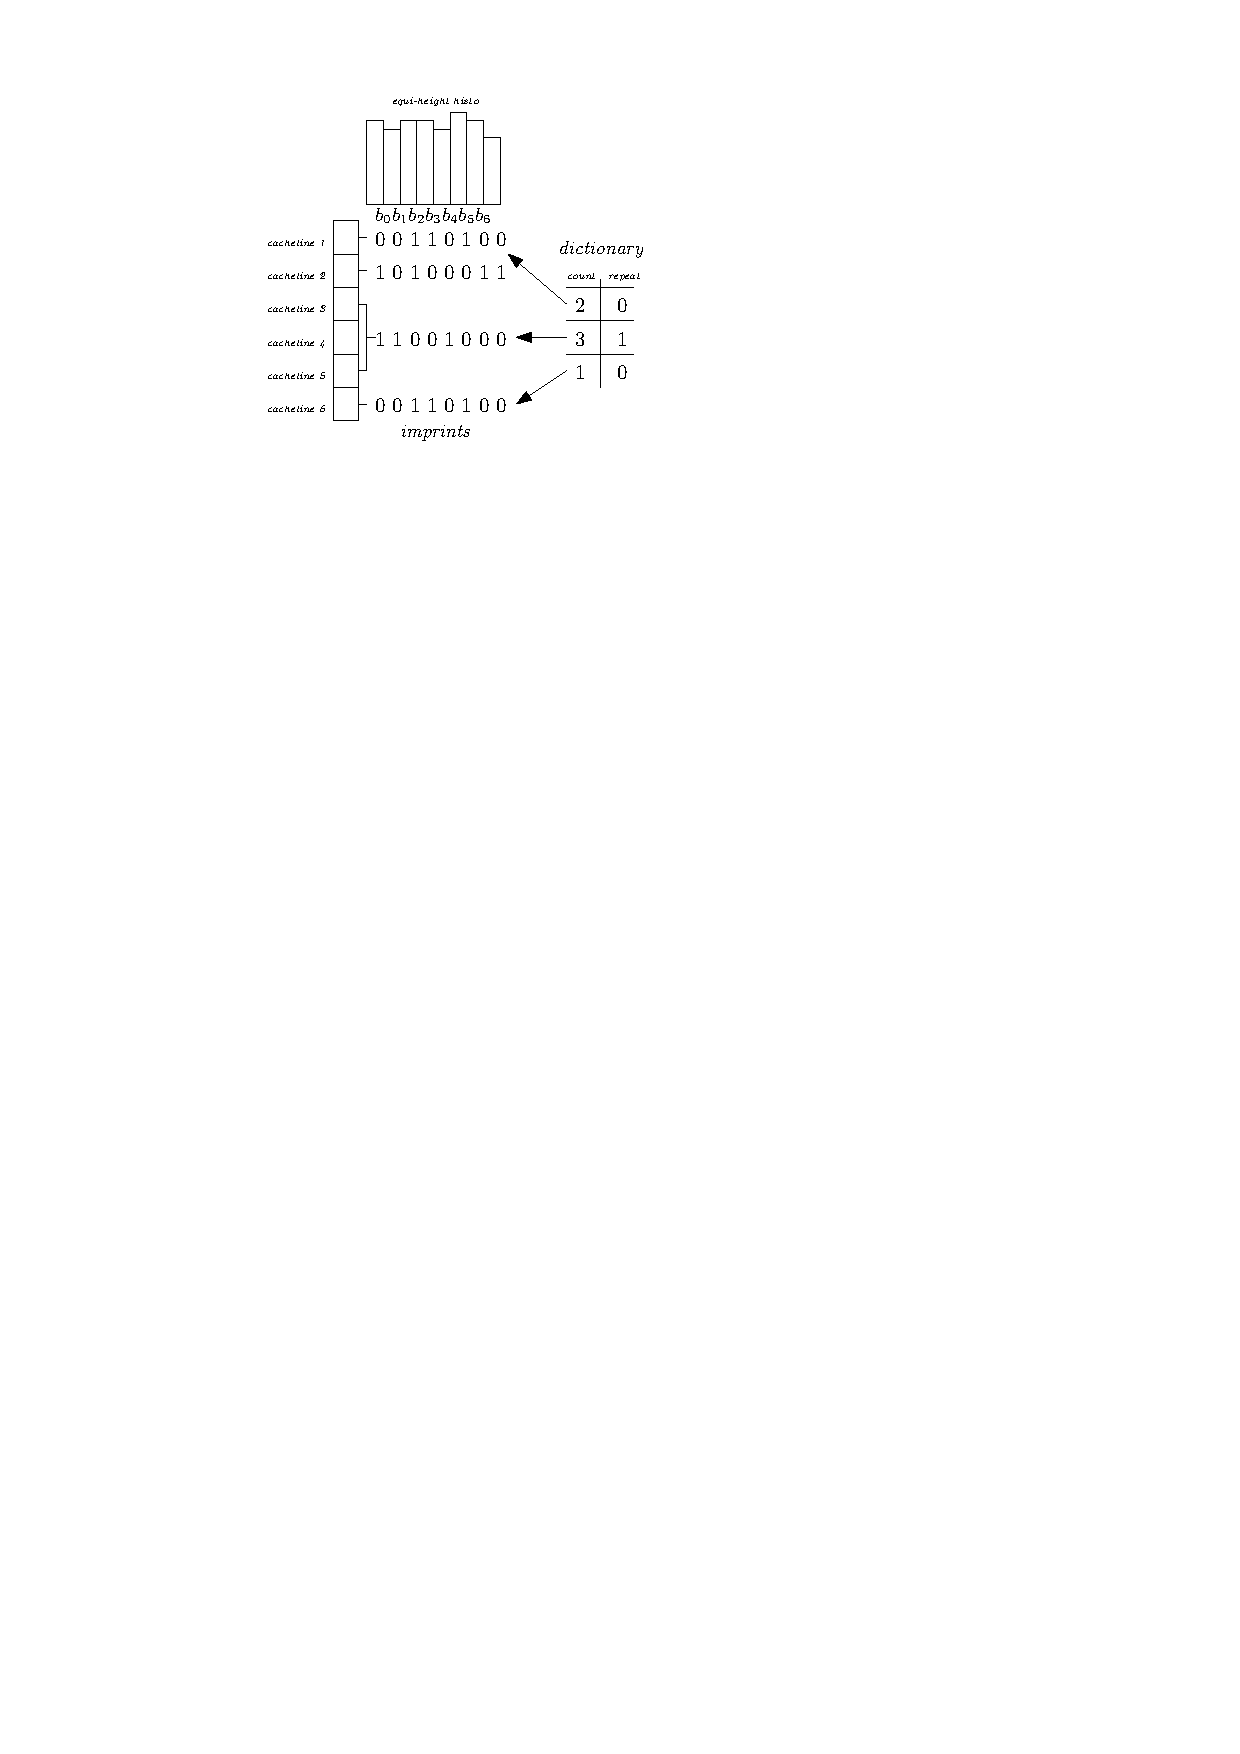
\includegraphics{imprints.pdf}
\end{center}
\caption{A Column Imprint Index\label{fig:imprints}}
\end{figure}

Figure~\ref{fig:imprints} gives an overview of the index structures. Given a column with values from
domain $\mathbf{D}$, an imprint index is constructed by first taking a small
sample to approximate a histogram of a few (typically 64 or less) equal-height
bins. These bins are used to derive the {\em boundaries} $b_i$ to be used to mark the range
each bit in the imprint covers (top part of Figure~\ref{fig:imprints}).  The entire column is
then scanned, and for every cacheline of data, a bit-vector is created. The 
bits in each bit-vector correspond to the bins of the histogram. A bit is set if at least one value in 
the cacheline falls into the corresponding bin. The resulting bit-vector is an imprint of the
current cacheline that describes which buckets of the approximated
histogram the values of the cacheline fall into. As shown in Figure~\ref{fig:imprints}, an imprint does
not have only one bit set per position, but as many bits as are needed
to map all distinct values of a cacheline. The collection of
all the resulting imprints form a unique {\em Column Imprint}. Consequently,
by examining the imprints of a column, the execution engine 
can decide -- in a cacheline granularity -- which parts of the column
data are relevant to the query predicates, and only then fetch them
for further processing. Contrary to previous work, a column imprint is a
non-dense bit indexing scheme, i.e., only one bit is set for all equal values
in a cacheline, instead of the traditional approaches of bitmaps where each
data point is always mapped to a different bit.

To reduce the memory footprint of imprints, a simple but powerful compression scheme is used.
Consecutive and identical imprints are compressed together and annotated with a counter.
The right side of Figure~\ref{fig:imprints} shows a small dictionary example. The count
column counts how many consecutive cachelines have unique imprints
(i.e., one imprint per one cacheline), or how many consecutive cachelines share the same imprint
(i.e., one imprint per many cachelines). The repeat column marks
the one-to-one relationship between cachelines and imprints ({\em repeat=0}), or the many-to-one
({\em repeat=1}). This compression exploits
the empirical observation that data suitable for secondary indexing
exhibits, in the cacheline level, some degree of clustering or partial
ordering. {\em Column imprints} are designed such that any clustering or partial
ordering is naturally exploited without the need for extra parameterization. 

\begin{algorithm}[t]
\begin{tabbing}
{\bf for} \=each cacheline\\
   \>{\bf for} \=each value $v$ in cacheline\\
        \>\>$i$ = \textbf{\textit{find\_bin}} ($v$)\\
        \>\>set $i$-th bit in current imprint\\
    \>{\bf if} current imprint $\equiv$ previous imprint\\
     \>\> compress and update dictionary
\end{tabbing}        
\caption{Create Column Imprints\label{algo:create}}
\end{algorithm}

\begin{algorithm}[t]
\begin{tabbing}
{\bf set} \=mask $m$ for range query $[low,high]$\\
{\bf for} each imprint $imp$\\
    \>{\bf if} \=$(imp\ \&\ m)\ \not=\ 0$\\
    \>\>{\bf for} \=each value $v$ in cacheline\\
    \>\>\>\textbf{\textit{check if}} $v\in [low,high]$
\end{tabbing}        
\caption{Query Column Imprints\label{algo:query}}
\end{algorithm}

Algorithms~\ref{algo:create} and~\ref{algo:query} provide a high level overview of the process to
create and query imprints. The creation process is a single scan over the data, where
for all values in a cacheline the function \textbf{\textit{find\_bin}} is invoked to determine which
bit in the imprint has to be set. This function call\footnote{implemented as a macro to avoid function call
overhead costs} is the time-dominant operation for Algorithm~\ref{algo:create}. Function \textbf{\textit{find\_bin}}
performs 64 comparisons of the form $v > b_i$ and it is exactly the part of the code that will be vectorized
in the next section.

Similarly, for the query Algorithm~\ref{algo:query}, the process starts by scanning each imprint $i$ and comparing
it with a mask bit-vector $m$. Mask $m$ has all bits that fall between the query range $[low,high]$ set,
i.e., $m[i] = 1$ if $low<b_i<high$. If imprint $imp$ and mask $m$ have common bits set, then the cacheline has to
be examined further for qualifying values and for rejecting false positives. This operation, denoted as
\textbf{\textit{check if}} in Algorithm~\ref{algo:query} is the most time consuming part of querying, and it will
be the subject of speeding up through vectorization in the next section.

For a complete presentation of {\em Column Imprints} and a detailed explanation of each algorithm we refer the
reader to~\cite{DBLP:conf/sigmod/SidirourgosK13}.


\section{Vectorized Column Imprints}\label{sec:concept}

For completeness of the presentation in this paper, we include the time dominant code snippets
of the scalar implementation of the imprints algorithms, as identified in the previous section and
described in details in \cite{DBLP:conf/sigmod/SidirourgosK13}. This work is about substituting these critical
snippets of code in the imprints creation and querying algorithms in order to enable advanced vectorization
optimizations.  

\subsection{Imprints Creation}
The performance-critical part of imprints creation is the histogram bin assignment for each value from the column data,
i.e., the code for \textbf{\textit{find\_bin}} function. Especially for wide imprints, it seems intuitive to implement a non-recursive binary search in the histogram boundary array $b[\ ]$ to determine the correct bin $i$, such that $v > b_i$
and $v<b_{i+1}$. However, the large amount of branching required makes this solution slower than a ``brute-force'' approach,
where all boundaries $b_i$ are checked against the input value, regardless the outcome, and all comparison results are summed up. The result is the bin index of the respective value $v$. The following pseudo-code illustrates this approach:

\begin{lstlisting}[language=c]
int res = 0;
for (int i; i < length(b); i++)
  res += v > b[i];
\end{lstlisting}

Vectorization of this approach is straightforward, depending on the input value type width (8, 16, 32 or 64 bits), we can ask
the CPU to perform many (up to 64 for AVX-512) value-to-bin boundaries comparisons in a single SIMD instruction. This works
because AVX comparison operators, for example \texttt{\_mm256\_cmpgt\_epi32}, will return a vector where each element is set
to $-1$ for each of the comparisons that evaluate to ``true''. These result vectors can then be summed up to yield the
bin boundary index.

\begin{figure}
\begin{center}
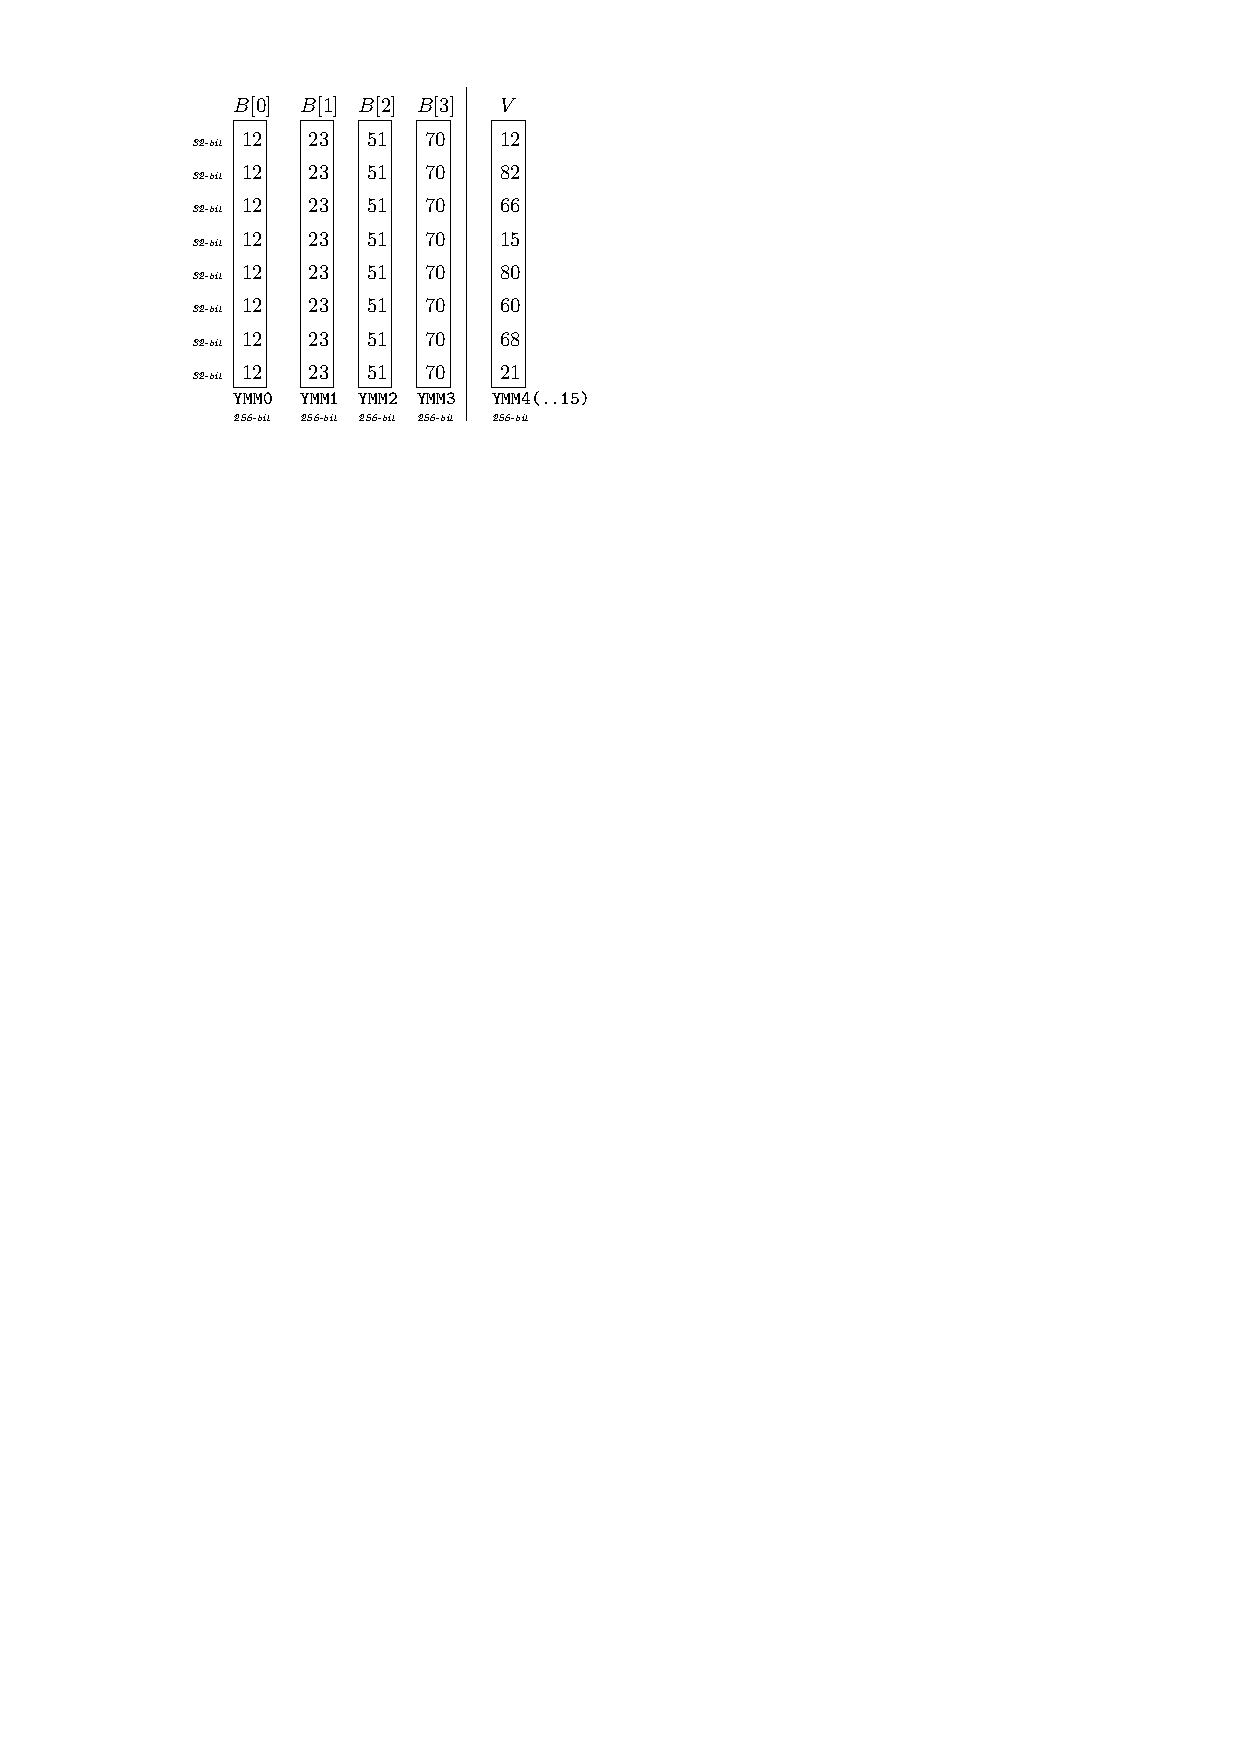
\includegraphics{simd_ex.pdf}
\end{center}
\caption{SIMD registers for imprints creation\label{fig:simd_ex}}
\end{figure}

To illustrate this method, consider the following example. We assume 256-bit SIMD instructions, 32-bit integer input values, 
4-bit imprints, and 8 values per imprint. The histogram boundaries $b_i$ in this example are $b_0=12$, $b_1=23$,
$b_2=51$ and $b_3=70$. In a preparatory step, we compute SIMD vectors for all boundaries where all vector entries are set to the 
boundary value $b_1$ and store them in an array of vectors, denoted with $B$. We use uppercase variable names for SIMD 
vectors. This was found to be faster than creating the boundary vector $B$ ad-hoc, at the expense of some additional 
memory use. Figure~\ref{fig:simd_ex} shows the four boundaries $b_i$ stored in the four SIMD registers $B[0]$ to
$B[3]$, and the fifth SIMD register $V$ that contains the 8 values of the data block (cacheline) to be compared.
The values in $V$ will be compared simultaneously, using SIMD instructions, with one boundary value at a time.
Therefore, the vectorized bin boundary index computation proceeds as follows in four steps (SIMD comparisons):

\bigskip

\begin{tabular}{l|l|rrrrrrrr}
&$RES$             &  0 &  0 & 0 & 0 & 0 & 0 & 0 & 0 \\
&$V$             & 13 & 82 & 66 & 15 & 80 & 60 & 68 & 21 \\
\hline
1&$RES$+=($V$$>$$B[0]$)& -1 & -1 & -1 & -1 & -1 & -1 & -1 & -1 \\
2&$RES$+=($V$$>$$B[1]$)& -1 & -2 & -2 & -1 & -2 & -2 & -2 & -1 \\
3&$RES$+=($V$$>$$B[2]$)& -1 & -3 & -3 & -1 & -3 & -3 & -3 & -1 \\
4&$RES$+=($V$$>$$B[3]$)& -1 & -4 & -3 & -1 & -4 & -3 & -3 & -1 \\
\hline
&$RES=0-RES$&  1 &  4 &  3 &  1 &  4  & 3 &  3 &  1 \\
\end{tabular}

\bigskip

The subsequent step is to extract the individual entries from $RES$ and look up the bit pattern for that particular histogram bin. All retrieved bit patterns are OR-ed together, creating the final imprint for a particular data block. In this example, the four-bit imprint would be $1101$, since no entries fall into the second histogram bin. Furthermore, the resulting imprint needs to be checked against the imprint of the previous block of input values. This post-processing is not particularly performance-critical and we only use SIMD instructions for imprints
that are larger than 64 bits, as we will explain later in this section in more details. This example is also simplified, usually more than
eight values would be represented by an imprint. In this case, the imprint is the logical OR of the results of several runs of the described
method.

Note that the bin boundaries for eight input values are determined using only 9 SIMD instructions. Using the sequential method described above, 64 
individual comparison instructions would have been required to achieve the same result. As vector width increases over time, this ratio increases 
further. However, we have found that the performance of the bin index computation can be further increased by comparing the values against two
(and not more) histogram boundaries in each iteration. The following code snippet shows this optimization. For each iteration along the boundaries
array $B$, $V$ is compared (\texttt{cmpgt}) with \emph{two} boundary vectors and the outcome is added together, and then added to the total result. We suspect this to be due to the lack of a data dependency within the first two steps of calculation in this version. Intel's Haswell, Broadwell, and Skylake architectures can execute at most two 256-bit SIMD instructions per cycle, which suggests a two-stage pipeline for those instructions. Hence, by removing the data dependency, we can get at most two instructions completed per cycle. Analysis of performance counters confirmed that the code here reached this maximum. As we will see in the experimental results, the speedup of roughly 15x over the scalar code can probably be traced to this effect and implementation.

The following code snippet shows this optimization for 32-bit integer input values.

\begin{lstlisting}[language=c]
__m256i RES = _mm256_setzero_si256();
for (int i1=0, i2=1;
      i1 < length(B)-1; i1+=2, i2+=2) 
  RES = _mm256_add_epi32(RES, 
    _mm256_add_epi32(
      _mm256_cmpgt_epi32(V, B[i1]),
      _mm256_cmpgt_epi32(V, B[i2])));		
\end{lstlisting}

One limitation of this approach is that the number of histogram bin boundaries (and hence imprint length) is limited by the type of the input 
values. This is because a vectorized comparison operators returns comparison results of the same size in turn. If $V$ is of type
\texttt{char}, then we use \texttt{\_mm256\_cmpgt\_epi8} to compare the values to boundaries, hence we can address at most 127 when we accumulate
comparison results in $RES$. As a result, we cannot create 256-bit imprints for 8-bit values. This is not a big issue since it does not
make a lot of sense to create 256 bins for at most 256 distinct values, unless we are aiming at a one-to-one bitmap indexing structure.

\subsection{Imprints Querying}

Querying the vectorized imprints is very similar to the scalar version with two exceptions. The comparison of both outer and inner range boundary 
bit masks with the imprint entries uses vectorized instructions instead of simple bitwise logic operations. This is done to support larger
than 64-bit imprints. There are three possible outcomes of this comparison. First, the data values represented by the imprint has no overlap with 
the query range. In this case, the querying process simply advances to the next imprint. Second, there might be a match with only the bits of the
mask that are inclusively entirely inside the range query, in which case all values represented by the imprint satisfy the query predicate without
further checking. The interesting third case is when there is a partial overlap with the mask, which means that individual data values need to be 
compared with the range boundaries in order to determine which values satisfy the range query predicates. Here, SIMD operations are used to compare 
multiple values with the upper and lower query range boundaries. This comparison can be done in one instruction.

\begin{figure}
\begin{center}
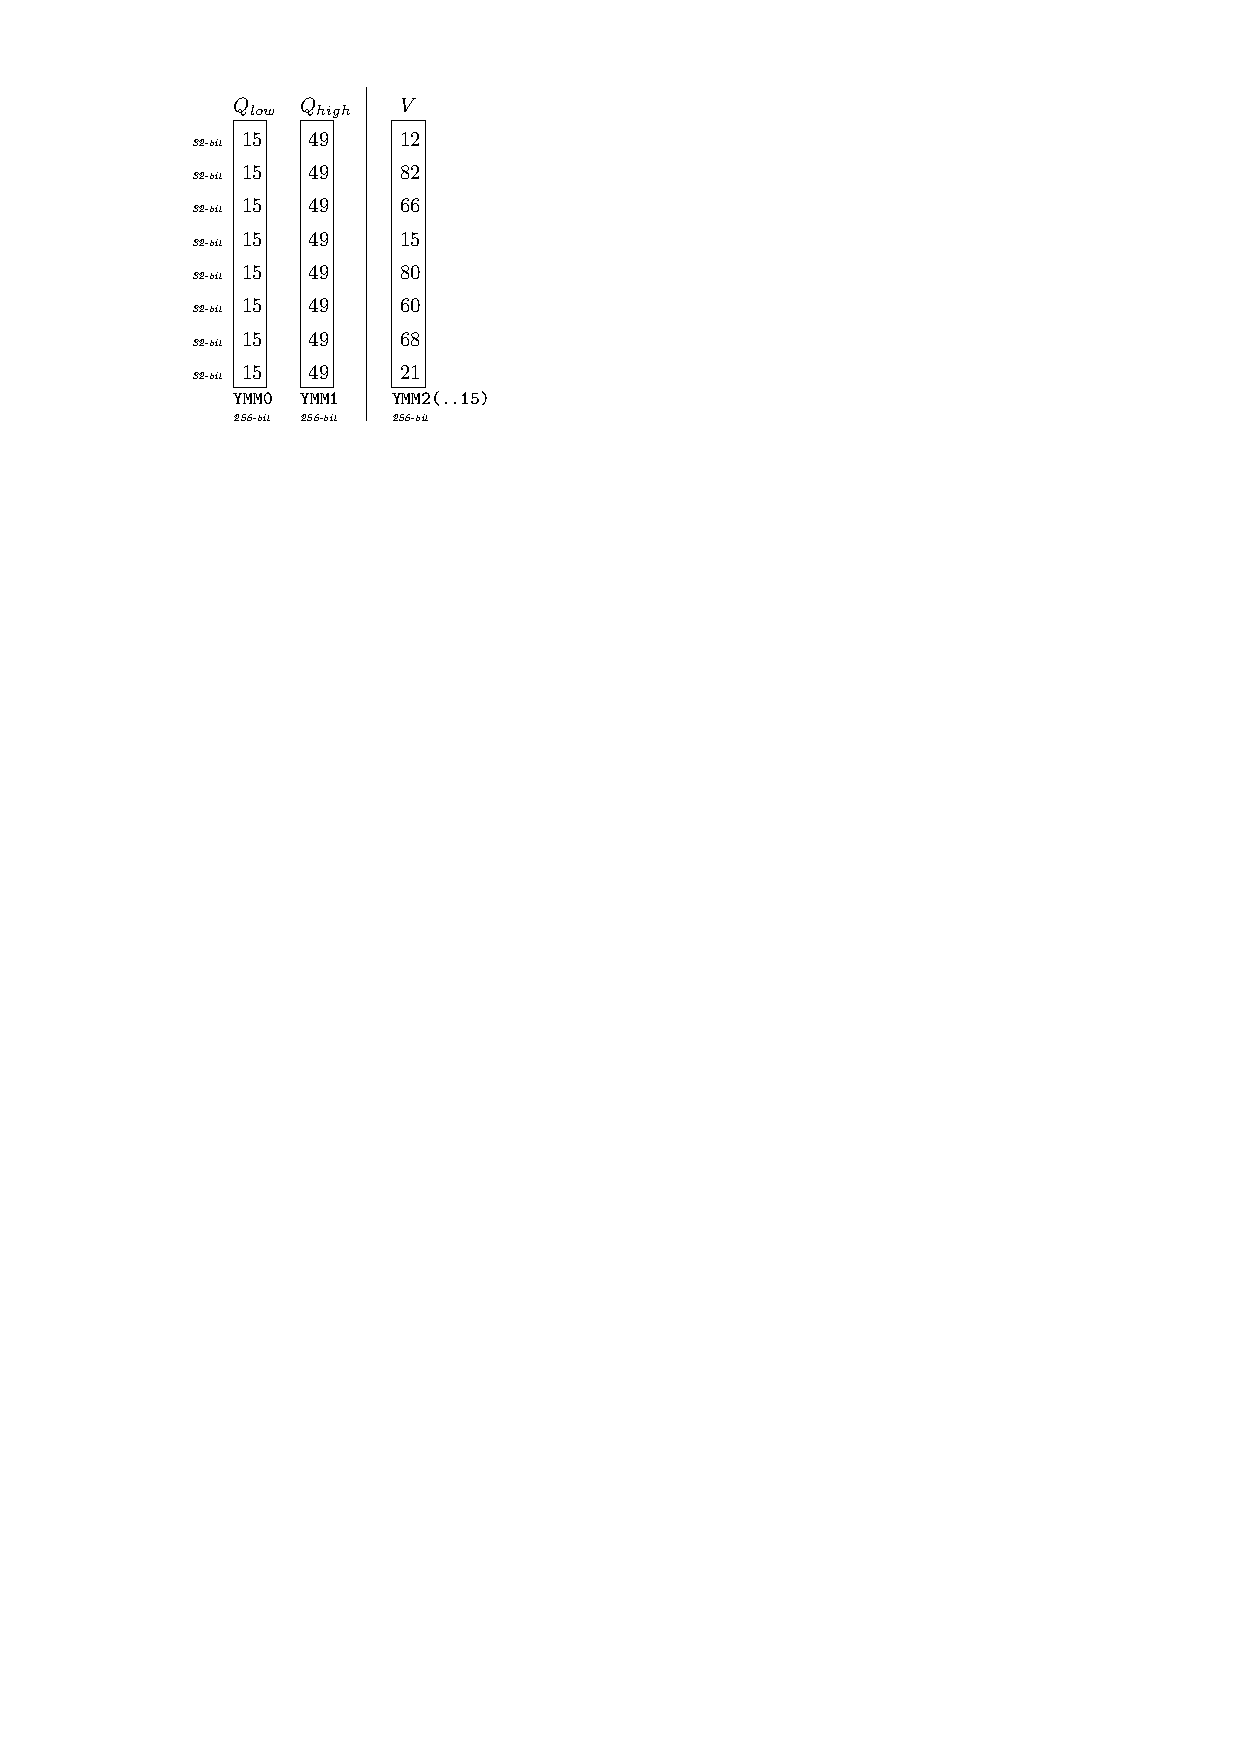
\includegraphics{query_ex.pdf}
\end{center}
\caption{SIMD registers for imprints querying\label{fig:query_ex}}
\end{figure}

Consider the same value array $V$ as in the example of the previous section. Also consider the range query $Q=[15,49]$. The
mask of this range query will be $0110$ since $Q_{low}=15$ is larger than $b_0=12$ and $Q_{high}=49$ is smaller than $b_3=70$.
The mask $0110$ has common bits set with the imprint of $V$ which was $1101$, thus the values of $V$ have to be examined one by one.
Figure~\ref{fig:query_ex} shows the two SIMD registers that store the $Q_{low}$ and $Q_{high}$ predicates of the range query.
Similarly, the next SIMD register holds the values of $V$ that will be compared with $Q_{low}$ and $Q_{high}$ in one go, using
vectorization.

The following code snippet shows the SIMD version of comparing imprints with the query mask Q\_MASK and checking the values against the low Q\_LOW and high Q\_HIGH ends of the query range for false positives.

\begin{lstlisting}[language=c]
if (_mm256_testz_si256(Q_MASK, IMPRINT)
 for (all values V in a data block)
   RES = _mm256_movemask_epi8(
          _mm256_sub_epi32(
           _mm256_cmpgt_epi32(V, Q_LOW),
           _mm256_cmpgt_epi32(V, Q_HIGH)));
\end{lstlisting}

The $RES$ variable has set the bits that correspond to the values of $V$ that satisfy the comparison with the low and high of the range query.
It is straightforward afterwards to identify the qualifying values from the $RES$ bit pattern.

\subsection{Larger Imprints}

Lastly, in order to support imprints larger than a 64-bit long word, we changed the type of an imprint from
\texttt{unsigned long} to a \texttt{\_\_mm256i}. Therefore, the bitwise operations had to be substituted with
SIMD instruction calls, such as \texttt{\_mm256\_or\_si256} for OR, and \texttt{\_mm256\_xor\_si256} for XOR.

Probably more interesting is the following code to check if two imprints have exactly the same bits set.

\begin{lstlisting}[language=c]
__m256i imprint1;
__m256i imprint2;
check = _mm256_xor_si256(imprint1,imprint2);
if (_mm256_testz_si256(check,check))
    # imprint1 is identical to imprint2 
\end{lstlisting}

The function \texttt{\_mm256\_testz\_si256} will return true if all bits in \texttt{check} are 0, but in order for
this to happen \texttt{imprint1} and \texttt{imprint2} have to have all bits set exactly the same.
Similarly, \texttt{\_mm256\_testz\_si256} function is used during the query process to check if an imprint has common
bits set with the query mask, where the mask is also an \texttt{\_\_mm256i} type. We refer the reader to our code 
repository\footref{repo} for further details about our implementation.

The changes presented in this section, from the scalar code to supporting SIMD instructions, accounts for a speedup up to 16 times.
In the next section we evaluate these changes, and examine the benefits of using more histogram bins, i.e., wider imprints, together
with larger than a cacheline data blocks. 

\section{Experiments}\label{sec:experiments}

To evaluate the performance of the vectorized version of imprints, we used a subset of the collection of datasets as in the original paper of
{\em Column Imprints}~\cite{DBLP:conf/sigmod/SidirourgosK13}. The data sets consist of 6,476 different columns, with a maximum number of
records of 600 millions, and contain integer and decimal types of various length. For a detailed overview of the data sets we refer
the reader to~\cite{DBLP:conf/sigmod/SidirourgosK13}. The dataset used for experiments is available on request.

We created a stand-alone implementation of SIMD imprints, which is available for download\footref{repo}. We compared our SIMD-enabled version of imprints with the original scalar implementation of imprints.

We are interested in mainly investigating the impact of two parameters. First, the bit width of the imprint (number of bins). Note that wider
imprints require more comparisons during index creation, thus we expected to have a slowdown as the number of bins increase, but always to be many 
times faster than the equivalent scalar version. The benefit of using larger bit-vectors for imprints is that the false positive ratio is reduced, 
thus having to check less values during query time. The second parameter we investigate is the number of encoded values per imprint, or in other 
words, the size of the block of data. This parameter will have an influence over the precision of the imprints. More values per block can lead to a 
smaller index size, but can lead to a negative impact on query performance, as more individual values need to be checked for false positives. In our
experiments, we vary the imprint size between 8 and 256 bits and the input block size (number of input values times their individual length) between
64 and 256 bytes. Other aspects of the imprints, such as the size and the compression percentage does not change with the SIMD-enabled version,
so we do not repeat these experiments. Note that the compression percentage has a fixed upper limit, and it is always the ratio between the size of
an imprint over the size of the data block. For each imprint configuration on each data column, we evaluate ten queries with even-spaced
selectivity between 0\% and 100\%.

All experiments were run on an Intel Core i7-6770HQ (``Skylake-H'') CPU clocked at 2.60~GHz. The system contained 32 GB of main 
memory. We also ensured that the files read are in the page cache before imprint creation.

All plots below show the average imprint creation or query time per 1,000 values over all data sets (and queries).  In addition, the standard error
is indicated as error bars.  For creation, ``values'' refers to input data values, for querying, it refers to imprint index entries. This is done
to allow a fair comparison between data sets of different sizes and different characteristics. For example, since the imprints index collapses
subsequent equal imprint entries using dictionary encoding, the data distribution has a direct impact on the scanning effort. In extreme cases
(a single constant value for the entire column), a single imprint entry can represent billions of data values. Hence this normalization.

\subsection{Imprint Creation}

\begin{figure}[t]
\begin{center}
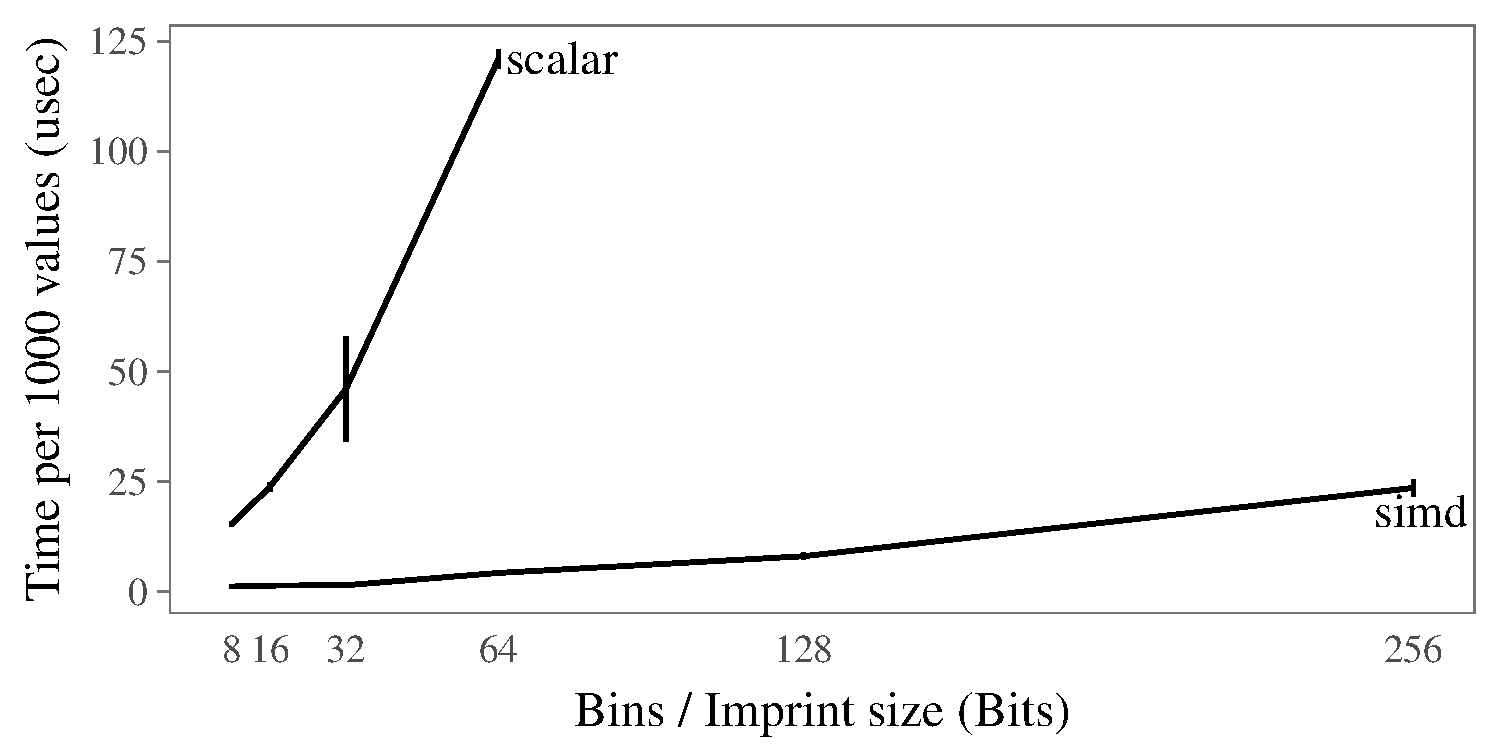
\includegraphics[width=\columnwidth,trim=0mm 0mm 0mm 0mm,clip]{scalebins1.pdf}
\end{center}
\caption{Imprint creation time vs. width.\label{fig:scalebins1}}
\end{figure}

We expect that the imprint size has a direct impact on index creation time, since every bit that is added requires additional comparison
operations. However, we also expect that the SIMD implementation described in this work will significantly outperform the optimized scalar
implementation. In the experiments in this section, we have varied the imprint size for both implementations in order to study these
expectations. 

Figure~\ref{fig:scalebins1} shows the outcome of this experiment. The scalar baseline and the SIMD implementation are shown as different lines. We can see how the time required to create imprints for 1,000 values scales linearly to the amount of bins and hence imprint size. We can also see
how the SIMD version greatly outperforms the scalar version, with the largest possible imprint size of 256-bits taking about as much time as the
scalar code for 16-bit imprints. For the 64-bit imprints, the scalar code required on average 120~\(\mu\text{s}\) per 1,000 values, while the SIMD implementation took only 4~\(\mu\text{s}\) with very low variance.

\begin{figure}[t]
\begin{center}
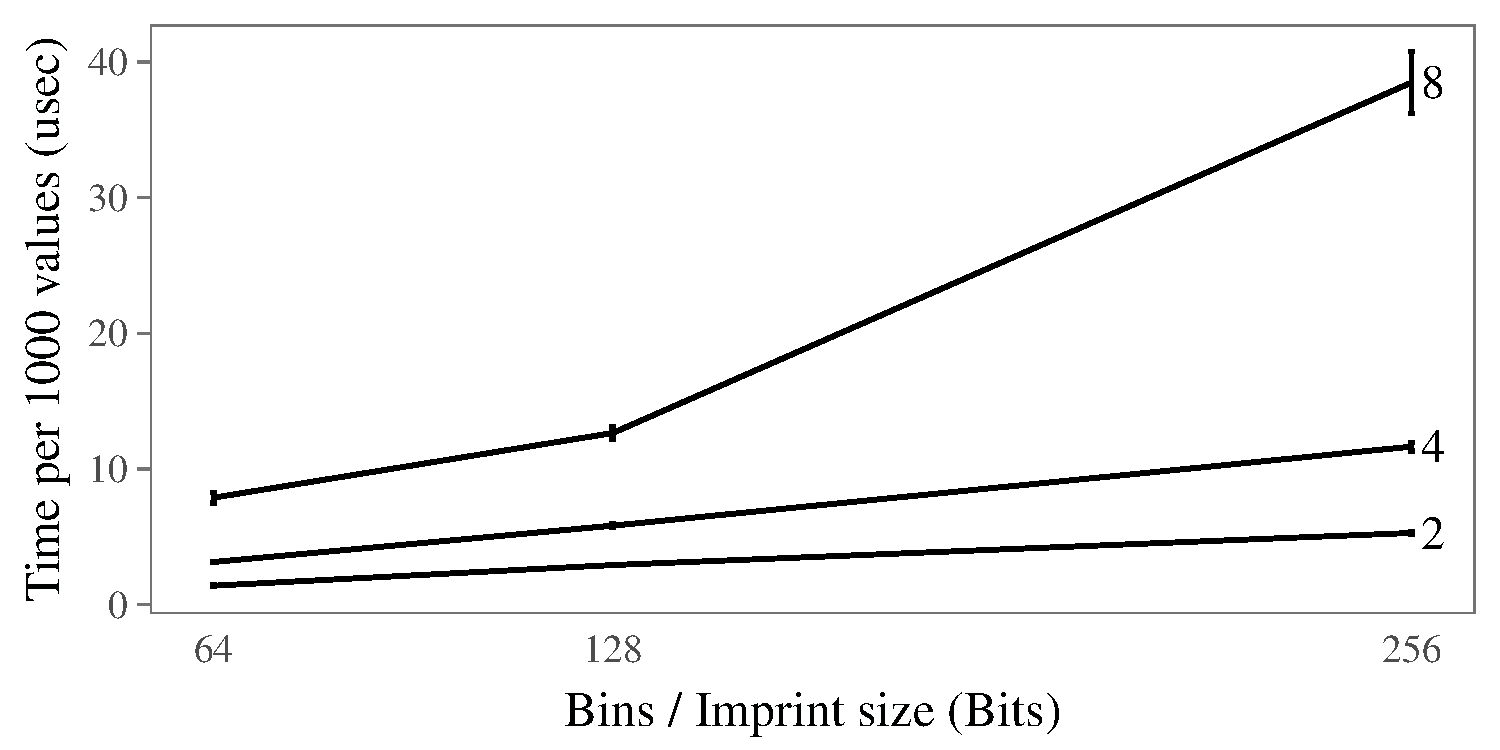
\includegraphics[width=\columnwidth,trim=0mm 0mm 0mm 0mm,clip]{typewidth1.pdf}
\end{center}
\caption{Imprint creation time for different value type widths (SIMD Only).\label{fig:typewidth1}}
\end{figure}

Drilling down, we further expect that the input type width has a significant impact on vectorized imprint creation time. For example,
for input data values of type \texttt{int16\_t}, 16 values can be boundary-checked in one SIMD instruction, while for \texttt{int64\_t} values only
4 comparisons are possible in a single instruction. Figure~\ref{fig:typewidth1} shows the imprint creation timing results (for the SIMD 
implementation only) by input data type width. As expected, we can see how data with 8 bytes input type width leads to the longest imprint
creation time, while the 2 bytes data is fastest. For 256-bit imprints, the 2 bytes values took on average of 5.3~\(\mu\text{s}\) per 1,000
values, while the 8 bytes type width took 38.5~\(\mu\text{s}\).

\begin{figure}[t]
\begin{center}
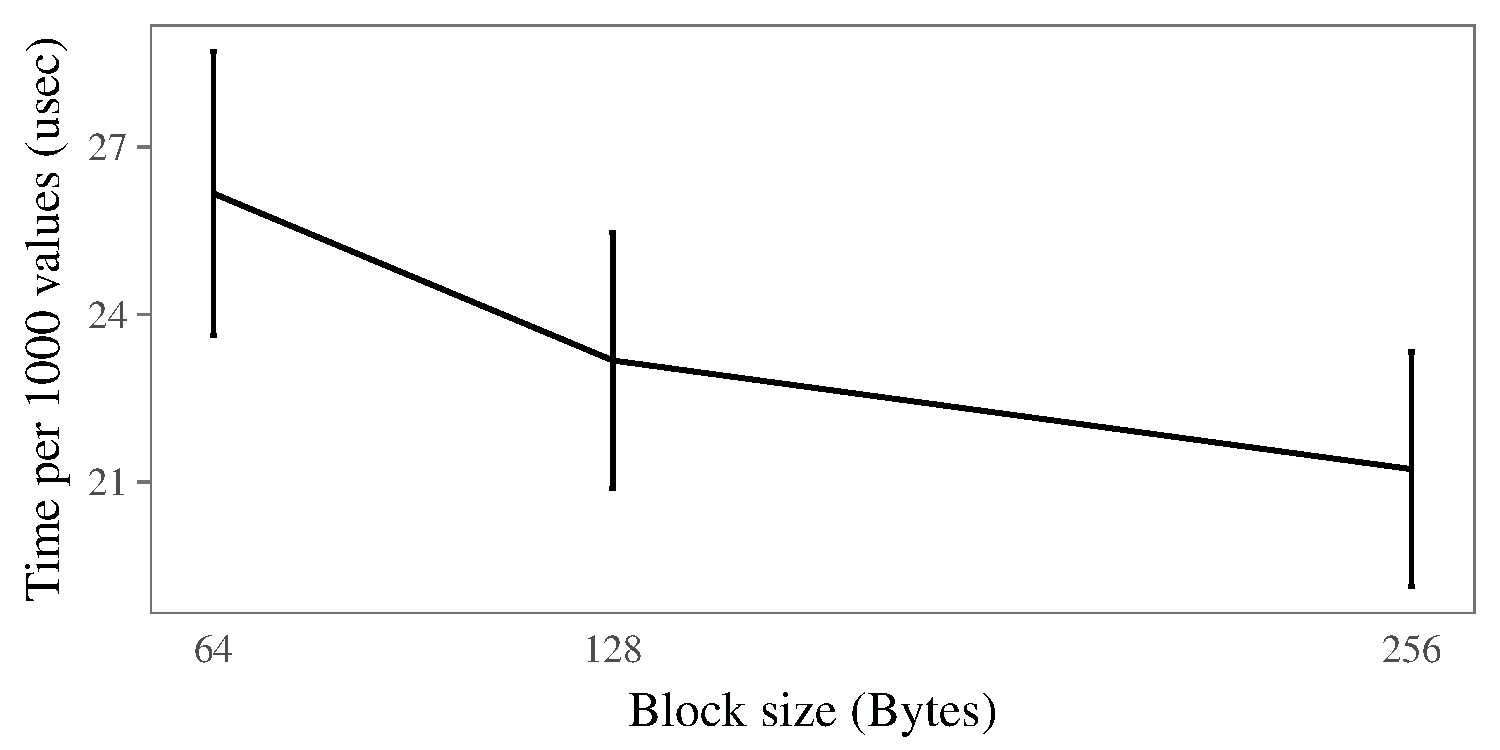
\includegraphics[width=\columnwidth,trim=0mm 0mm 0mm 0mm,clip]{block_size_bytes1.pdf}
\end{center}
\caption{Imprint creation time for different block sizes encoded (SIMD Only, 256 Bins).\label{fig:bytesperblock1}}
\end{figure}

Turning towards the second parameter, the amount of input data values per imprint entry, we expect that fewer values per imprint will improve
creation time since fewer imprint candidates need to be created and compared with the previous entry for dictionary compression purposes. For
this experiment, we have varied the number of input values per imprint between 8 and 128 in such a way that the input block size (the amount of input values multiplied by their type length) ranges between 64 and 256. Figure~\ref{fig:bytesperblock1} shows the results of this experiment. We can see how indeed the imprint creation time drops significantly if more data is encoded into a single value. However, a larger block size will
also lead to reduced precision, which has an adverse effect on query run time, which we will investigate next.

\subsection{Imprint Querying}

Querying performance is a trade-off between to extremes. On the one end, the imprint index is empty, requiring a full scan of the data values.
On  the other end, the imprint index is a one-to-one (bit-)mapping of the data. While both are technically valid, we are searching for a more
balanced  trade-off. This trade-off is controlled by imprint length and block size. 

\begin{figure}[t]
\begin{center}
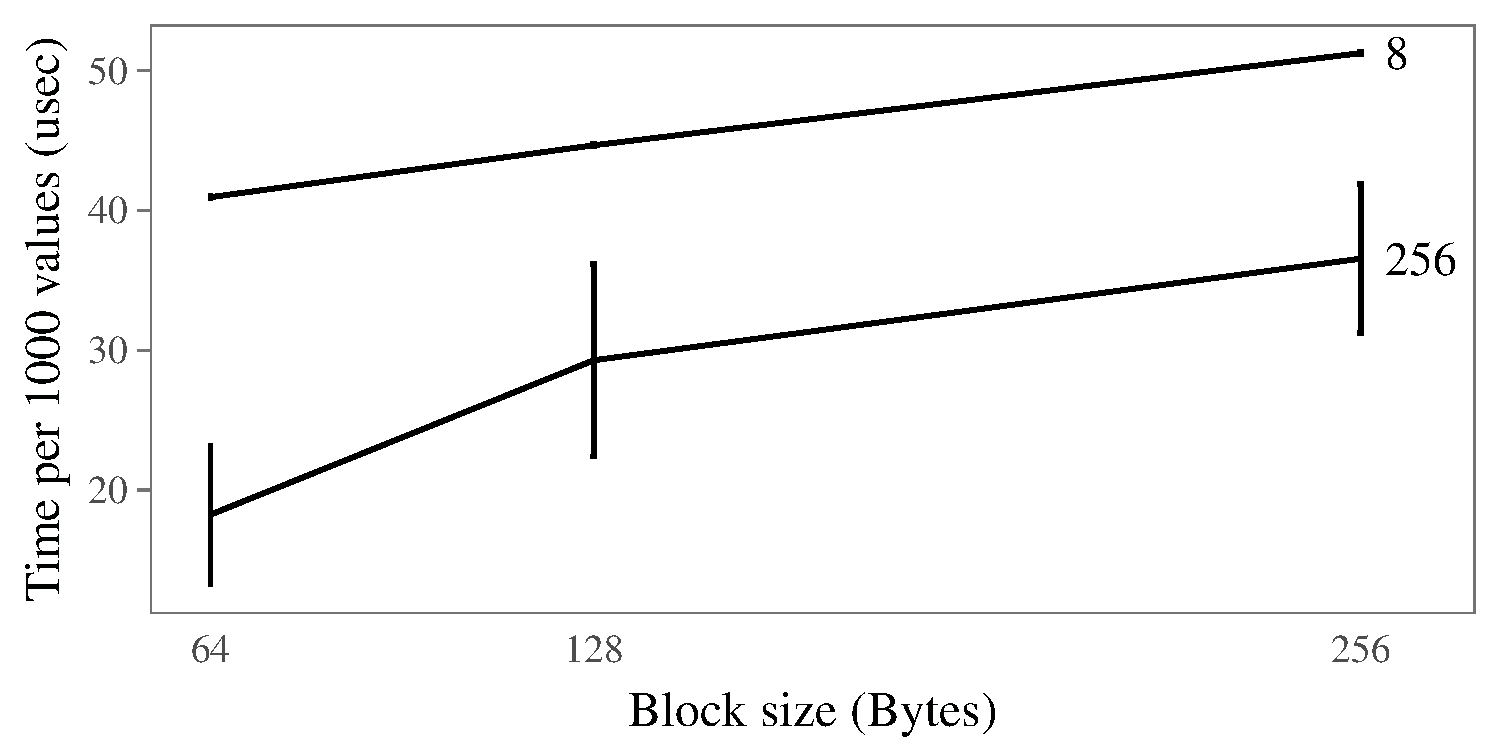
\includegraphics[width=\columnwidth,trim=0mm 0mm 0mm 0mm,clip]{qblocksize1.pdf}
\end{center}
\caption{Imprint querying time for different block sizes (SIMD Only).\label{fig:qblocksize1}}
\end{figure}

We expect that larger block sizes will decrease query performance (as more entropy is lost), but it is unclear by how much.
Figure~\ref{fig:qblocksize1} plots the time required to process 1,000 imprint index entries against increasing block sizes.
Two lines are shown, one for 8- and one for 256-bits imprint length. We see that query performance indeed decreases as block
size is increased, but (on average) at most linearly. It is very likely that query performance will degrade for even larger
block sizes, certainly if data values have to be fetched from disk.

\begin{figure}[t]
\begin{center}
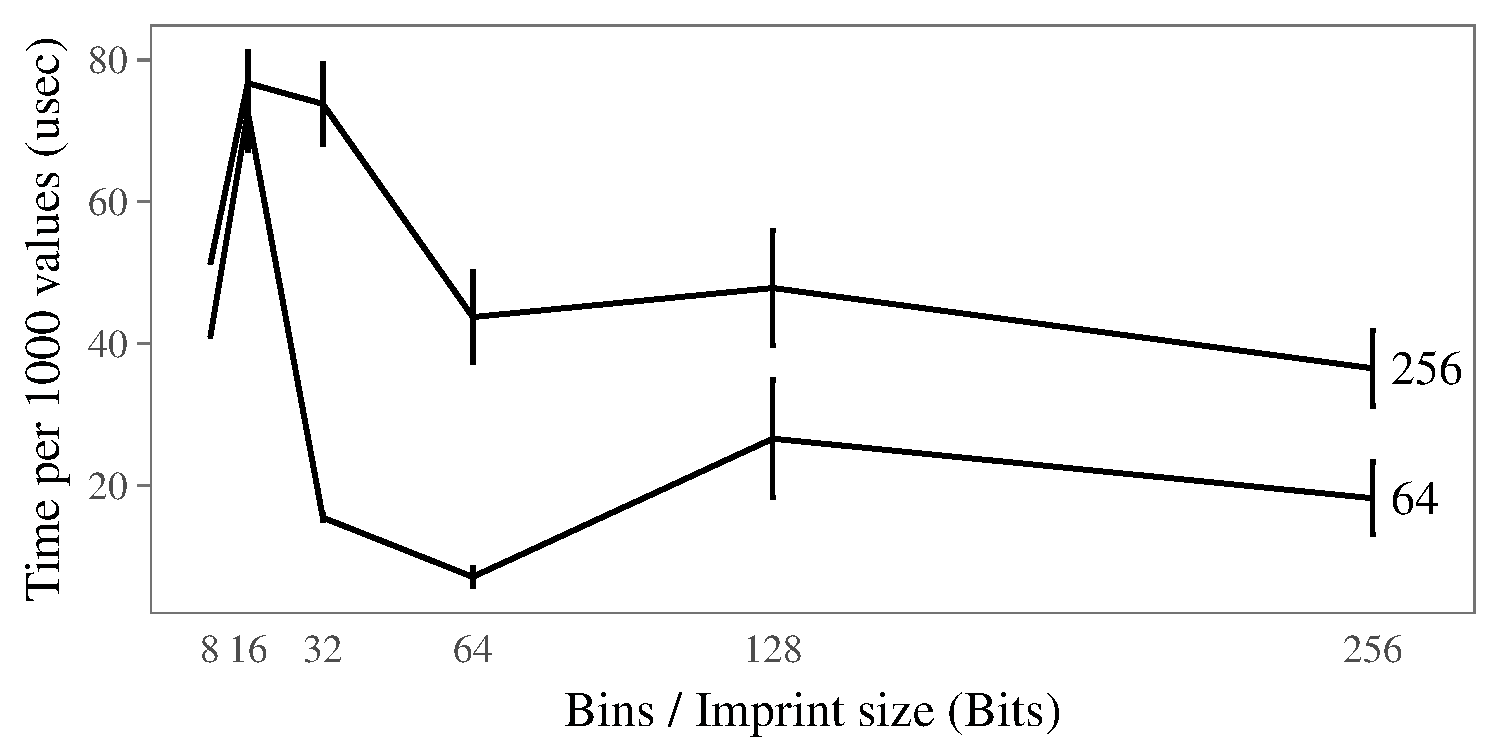
\includegraphics[width=\columnwidth,trim=0mm 0mm 0mm 0mm,clip]{qblocksize2.pdf}
\end{center}
\caption{Imprint querying time for different amounts of values encoded (SIMD Only).\label{fig:qblocksize2}}
\end{figure}

In the original imprints paper, a 8-to-1 relationship between data value bits and (before duplicate elimination) imprint bits was found to work
best. When scaling this up to larger imprints, we expect this relationship to still hold. Figure~\ref{fig:qblocksize2} shows a rather complex
behavior of the queries. However, the basic assumption that a 8-to-1 relationship between data and index still holds. For the 64 bytes block size,
we observe good performance for an imprint size of 64-bits. For the 256 bytes blocks, 256-bits imprints size showed the best performance, which
confirms our expectations. A similar result was found for the (not plotted) 128 byte block size with 128-bits imprints.

Overall, we argue that the experimental results show good scalability of imprint indexes thanks to the availability of vectorized instructions.

\section{Related Work}

There has been a large amount of previous work related to using SIMD vectorization to speed up analytical data management tasks.
Early papers demonstrated how existing implementations of relational operators could be sped up using SIMD
instructions~\cite{DBLP:conf/sigmod/ZhouR02}. Generally speaking, systems that use columnar or (data-)vectorized storage models
can benefit from a straightforward translation from scalar code implementing relational operators to the equivalent vectorized
code. 

A more thorough operator redesign was shown to be required to to fully take advantage of vectorized 
instructions~\cite{Polychroniou:2015:RSV:2723372.2747645}. The authors used selective load and store and scatter/gather operations available
in modern SIMD instruction sets as building blocks for new scan and join operators. Experimental results show that for example for low
selectivity, vectorized code can provide an approximately 10 times throughput improvement in scans. Overall, the authors found that
vectorization favors cache-conscious algorithms and that the speedup provided by vectorization is independent of other optimizations.

A paper comparing sort and hash join algorithms~\cite{DBLP:journals/pvldb/KimSCKNBLSD09} already reported the observation that sort-based join
algorithms scale near-linearly with the SIMD width. The paper also predicted that sort-based join algorithms are expected to show better
performance than hash-based approaches with a SIMD width of 512-bits or higher. This shows the relevance of the increased vector widths that
are now becoming available.

Data layout adaption is a third option apart from the previously discussed operator re-implementation and algorithmic redesign. One paper proposes
to adapt in-memory data layout in such a way that it is amenable to SIMD processing~\cite{Li:2013:BFS:2463676.2465322}. In such layout, every
SIMD word contains bits from a large amount of data values, which allows early pruning of data blocks in selections based on prefix comparisons
or improved look-up performance.

The overall research progression in transforming scalar code to vectorized could be described by the following chart with
representative references.

\begin{center}
\begin{tabular}{cr}
Operator Re-Implementation with SIMD Instructions & \cite{DBLP:conf/sigmod/ZhouR02} \\
$\downarrow$ & \\
SIMD-Aware Algorithm Design & \cite{Polychroniou:2015:RSV:2723372.2747645} \\
$\downarrow$ & \\
SIMD-Aware Data Layout Adaption & \cite{Li:2013:BFS:2463676.2465322}\\
\end{tabular}
\end{center}

\section{Conclusion \& Research Outlook}\label{sec:conclusion}

In this paper we have demonstrated that by substituting the expensive scalar code snippets of column imprints with the equivalent
single-instruction multiple-data code snippets, we can achieve a speed up of almost 16 times. The exercise of finding the equivalent
SIMD version is an interesting one, and requires some work to identify the correct code snippets to be changed. SIMD instructions
benefit from continues sequential loading, while control flow branching has to be avoided always. These observations makes the job
more challenging, and can lead to different index design choices. For example, we plan to investigate the possibility of dropping
altogether the compression features of {\em Column Imprints} (which require some if-else statement) in favor of non-interrupting
sequential loads (i.e., memory streaming) and bulk bit-wise comparisons. 

% we have this below in more detail
% Another option is to use the techniques from~\cite{DBLP:conf/sigmod/LangMFB0K16} to pre-computed candidate list output for all cases before
looking for false positives, thus splitting the process of uninterrupted bulk operations and conditional branching.

Another important aspect of our work is the expansion from 64-bit word registers to the equivalent 256-bit SIMD registers, and
therefore the increase of the imprints width. The, soon to come, AVX-512 which will support 32 512-bit SIMD registers will allow
for even more performance boost for imprints.

However, the interesting observation is that not only {\em Column Imprints} but other bit-vector based techniques can benefit from SIMD
instructions. We believe that there is interesting work to be done here, and we intend to extend this work to other techniques such as
WAH bitmap compression~\cite{Wu:2006:OBI:1132863.1132864}. 

Another promising direction to speed up querying is to pre-compute all possible result offset vectors similar
to~\cite{DBLP:conf/sigmod/LangMFB0K16}. For example, if the values $(1,5,6,3)$ are checked for the range query $[2,5]$, only the second and last
entry are true positives. For this case, the pre-computed vector $(\mathtt{NULL}, 0, \mathtt{NULL}, 1)$ can be looked up, and then add the base
index for this block of values, say $42$, using vectorized instructions, thus we have efficiently created the output candidate list
$(\mathtt{NULL}, 42, \mathtt{NULL}, 43)$. AVX has a feature to control which elements from a SIMD register should be copied into contiguous
main memory, making final assembly of the result efficient as well.

A final thought on research outlook is that, although now we are successfully trying to adjust existing index structures to the SIMD era,
we should start designing new indexes that have native support for vectorization. Complex compression, multiple branching, and other structures
that aimed at loading less data in the CPU might be abandoned for the use of SIMD instructions such as \_mm256\_stream\_load\_si256 that allow
stream loading with non-temporal memory hints. The benefits of such bulk loads may overweight the benefits of less data transfer through control
flow statements.

\begin{acks}
Stefan Manegold of the CWI Database Architectures Group optimized the scalar imprints code.
This work was partially funded by the Netherlands Organisation for Scientific Research (NWO),
project ``Capturing the Laws of Data Nature'' (M\"uhleisen).
\end{acks}

\bibliographystyle{ACM-Reference-Format}
\bibliography{sigproc} 
\balance

\end{document}
